%%%%%%%%%%%%%%%%%%%%%%%%%%%%%%%%%%%%%%%%%%%%%%%%%%%%%%%%%%%%%%%%%%
%%	    mmm  mmmmmm mm   m        m    m mmmmmm   mmm	%%
%%	  m"   " #      #"m  #        #    # #      m"   "	%%
%%	  #   mm #mmmmm # #m #        #    # #mmmmm #m""#m	%%
%%	  #    # #      #  # #  """   #    # #      #    #	%%
%%	   "mmm" #mmmmm #   ##        "mmmm" #mmmmm  #mm#"	%%
%%								%%
%%                                                              %%
%%                                                              %%
%%      Grundlagen der Elektrischen Netzwerke, UE               %%
%%      Gruppe 5, Team F                                        %%
%%      Authors: Severin Wolf, Maximilian Seidler.              %%
%%%%%%%%%%%%%%%%%%%%%%%%%%%%%%%%%%%%%%%%%%%%%%%%%%%%%%%%%%%%%%%%%%
\documentclass[a4paper]{article}
\usepackage{amsmath}
\usepackage[utf8]{inputenc}
\usepackage[T1]{fontenc}
\usepackage[english]{babel}
\usepackage{geometry}
\usepackage{graphicx}
\usepackage{tikz}
\usepackage{listings}
\geometry{a4paper,left=3cm,right=2cm, top=2cm, bottom=2cm} 
\usepackage[EFvoltages, european, straightvoltages]{circuitikz}

%tikz
\ctikzset{resistor = european}
\usetikzlibrary{decorations.pathreplacing}

%no paragraph indent
\setlength{\parindent}{0pt}

%for math, that does not fit
\renewcommand*{\arraystretch}{1.3}
\newcommand\scalemath[2]{\scalebox{#1}{\mbox{\ensuremath{\displaystyle #2}}}}

\newcommand\blfootnote[1]{%
	\begingroup
	\renewcommand\thefootnote{}\footnote{#1}%
	\addtocounter{footnote}{-1}%
	\endgroup
}

% upright differenzial symbol with good spacing included!!!
\makeatletter
\providecommand*{\diff}%
	{\@ifnextchar^{\DIfF}{\DIfF^{}}}
\def\DIfF^#1{%
	\mathop{\mathrm{\mathstrut d}}%
		\nolimits^{#1}\gobblespace
}
\def\gobblespace{%
	\futurelet\diffarg\opspace}
\def\opspace{%
	\let\DiffSpace\!%
	\ifx\diffarg(%
		\let\DiffSpace\relax
	\else
		\ifx\diffarg\{%
			\let\DiffSpace\relax
		\else
			\ifx\diffarg\{%
				\let\DiffSpace\relax
			\fi\fi\fi\DiffSpace}

\begin{document}
\pagestyle{empty} \enlargethispage*{25cm}\samepage{
\vspace*{-3cm}
\begin{center}
\begin{minipage}[!h]{16cm}
\hspace*{0.2cm}

\includegraphics[width=3.3cm]{./Figures/igte_logo}
\begin{tabular}{p{8cm}}
\vspace{0.2cm}
\centering{
\Large Institute of Fundamentals and Theory in
 Electrical Engineering\\
Graz University of Technology\\
~\\}
\end{tabular}

\includegraphics[width=3.3cm]{./Figures/TUG_logo}
\end{minipage}
		\Large
		\textbf{Fundamentals of Electrical Circuits} \vspace*{0.5cm}\\
		\textbf{6. Homework}\\
		Fourier Series
		\vspace*{0.5cm}
		
		\large
		29. April 2021
	\end{center}}
	\vspace*{1cm}
	
	%%%%%%%%%%%%%%%%%%%%%%%%%%%%%%%%%%%%%%%%%%%%%%%%%%%%%%%%%%%%%%%%%%%%
	%%%%%%%%%%%%%%%%%%%%%%%%%%%%%%%%%%%%%%%%%%%%%%%%%%%%%%%%%%%%%%%%%%%%
	
\textbf{Every plot you create should also include the input signal.}
	\begin{enumerate}
		\item Derive the Fourier Series expression for the periodic voltage function given in figure \ref{fig:input}. Determine the \textbf{values} of the coefficients for the fundamental wave and the first four (\textbf{nonzero}) higher harmonics \textbf{numerically} with \textsc{Matlab} by using the command \texttt{trapz}.
		 (\textbf{1.5 Points})
		 
		\item Plot these five individual waves and determine the frequency for each of them. Also plot the sum of these waves. (\textbf{1 Point})
		
		\item Plot the Fourier Series for the first 250 waves. Does the Fourier Series converge towards the given input signal? (\textbf{0.5 Points})
		
		\item A student wants to use the lowpass-filter in Figure~\ref{fig:filter} to filter out frequencies higher than the fourth higher harmonic (\textbf{nonzero}) from the input signal. For the cut-off frequency they therefore use the frequency of this fourth higher harmonic. Determine the capacity $C$ of the capacitor for which this requirement is fulfilled. (\textbf{0.5 Points})
		
		\item Determine the transfer function $\underline{H}(j\omega) = \frac{\underline{U}_\text{out}}{\underline{U}_\text{in}}$ and use it to determine the output signal $u_\text{out}(t)$. Use the Fourier Series of Task 3 for that. \\
		Plot the output signal and the summed signal of Task 2 in one diagram. Do indeed only the desired frequencies remain? What could be the reasons for the differences between these two signals?\\ (\textbf{1.5 Points})
	\end{enumerate}

	\subsection*{Values:}
	$R = \frac{5000}{\pi}~\Omega$ \qquad $T = 40~ms$\\
\begin{figure}[!htb]
\begin{minipage}{0.55\textwidth}
	\centering
	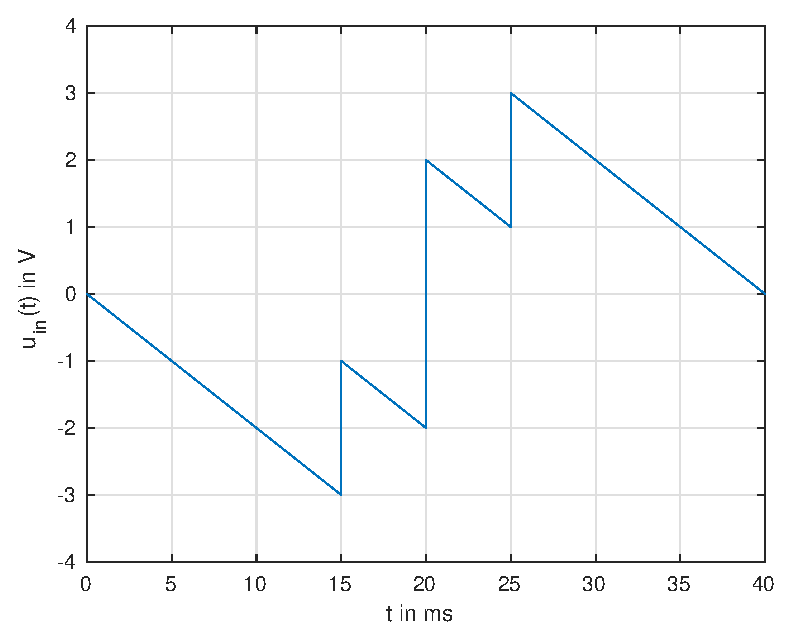
\includegraphics[width=1\textwidth]{./Figures/inputsignal.eps}
	\caption{Input Signal}
	\label{fig:input}
\end{minipage}\hfill
\begin{minipage}{0.39\textwidth}
	\centering
	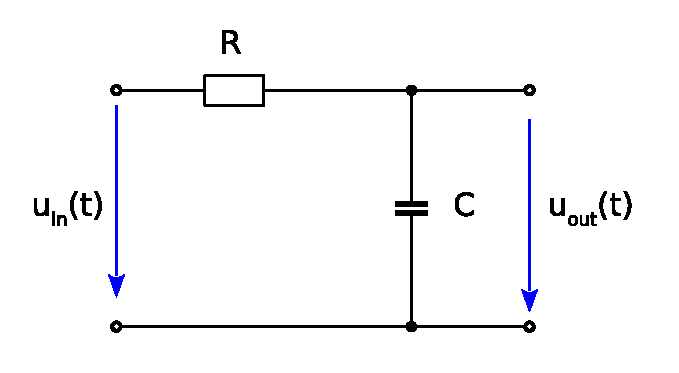
\includegraphics[width=1\textwidth]{./Figures/filter.eps}
	\caption{Filter-Circuit}
	\label{fig:filter}
\end{minipage}
\end{figure}
	\blfootnote{Deadline: 6.5.2021; Presentation: Team 6}

\clearpage
\section{Solution}
\subsection{Fourier Series - Numerical solution}
The input signal, as seen in Figure \ref{fig:input}, fulfilles all dirichlet conditions and
therefore,
it can be written as
\[
  f(t) = a_{0} + \sum_{k=1}^{\infty} (a_{k}\sin k\omega t + b_{k}\cos k\omega t)
.\] 
$a_{0}$ and all $a_{n}$ are going to be zero, because $f(t) = -f(-t)$. The cosine coefficients
need to be calculated, which will be done numerically, using an appromation of the integral
\[
  b_{k} = \frac{2}{T}\int_{0}^{T} f(t) \sin(k\omega t) \diff t
.\] 
For that, we are going to use the trapezoidal rule. Matlab has a standard function for that, named
'trapz'. The following coefficients for the first four harmonics have been calculated with the
script in the matlab section.
\[
  b_{1} = -2.1729, \quad b_{2} = 0.63562, \quad b_{3} = -0.1236, \quad b_{4} = 0
.\] 
Their corresponding frequencies can be calculated via $f_{k} = k \frac{1}{T}$. That yields:
\[
  f_{1} = \frac{1}{40}Hz, \quad f_{2} = \frac{1}{20}Hz, \quad f_{3} = \frac{3}{40}Hz, \quad
  f_{4} = \frac{1}{10}Hz
.\] 
The plot for those five harmonics looks like the following
\begin{figure}[h!]
  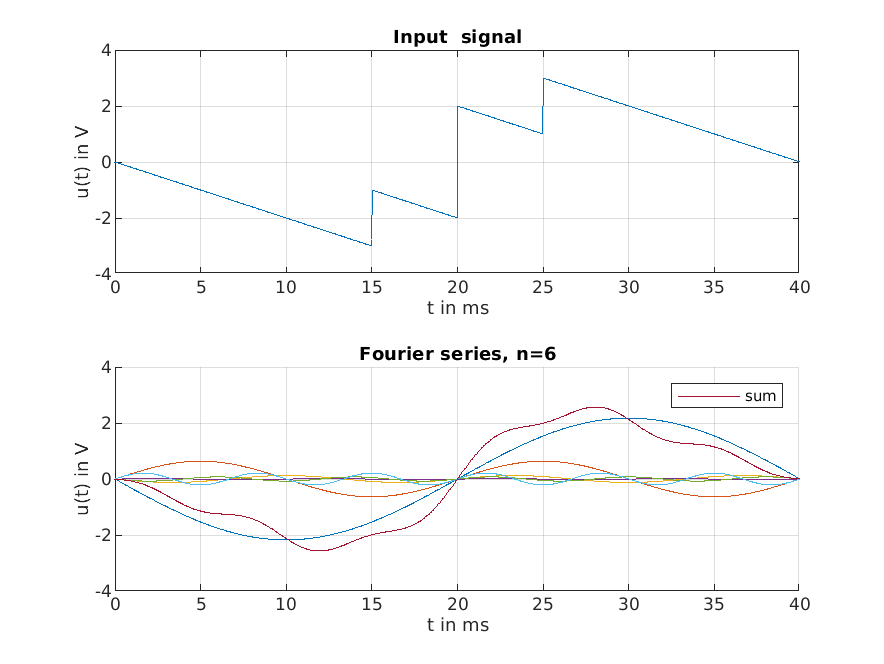
\includegraphics{"./Figures/fourier_n5.png"} \centering
  \label{fig:fourier5}
  \caption{first 5 harmonics}
\end{figure}
\clearpage
As one can see, the fourier series for $f(t)$ with $n=5$ is not yet an acurate approximation of
the input Signal. Let's increase $n$ to  $250$ and plot it again. 
\begin{figure}[h!] \centering
  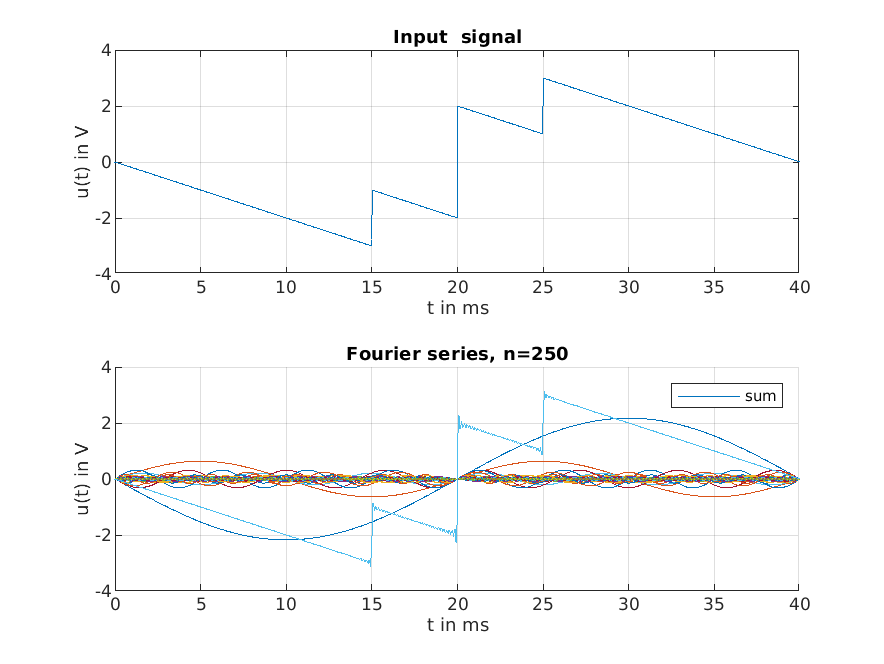
\includegraphics{"./Figures/fourier_n250.png"}
  \label{fig:fourier250}
  \caption{first 250 harmonics}
\end{figure}
\end{document}
We get a quite satisfying result. Should we increase n even more, our result will get even better.
But does it converge to $f(t)$? The answer is sort of. At points $t$, where  $f(t)$ is continous,
yes the fourier series for converges to $f(t)$. But at points, where $f(t)$ is discontinous, meaning
that there is a conditional jump, the fourier series converges to  $\frac{f(x+) + f(x-)}{2}$.
